
% additional usepackage{beamerthemeshadow} is used
\documentclass{beamer}
%\usepackage{beamerthemeshadow}

\usepackage{lmodern} % Font
\usepackage[T1]{fontenc} % Can use danish characters
\usepackage[utf8]{inputenc} %input encoding. Can be used on Linux, Mac and Windows         
\usepackage[english]{babel} %Split words accoding to English

%Standard path to search for pictures
%--------------------------------------------------
%\begin{figure}[hbtp]
%\centering
%\includegraphics[width =0.9 \textwidth]{filnavn-for-png}
%\caption{Titel}
%\label{fig:referenceNavn}
%\end{figure}
%--------------------------------------------------

\usepackage{graphicx}
\usepackage{subcaption}
\usepackage{float}

%Paths the pictures can be located
\graphicspath{
	{../Figures/}
	{Figures/}
}

% URL links and color for page numbers, links, cites, etc.

\usepackage{color} 
\usepackage{hyperref}
\hypersetup{ 
	colorlinks	= true, 	% false: boxed links; true: colored links
    urlcolor	= blue,		% color of external links
    linkcolor	= black, 	% color of page numbers
    citecolor	= blue,		% HERE
}

% \url{www...}

\begin{document}

\title{Version control and GitHub}  
\author{Rasmus Bækgaard}
\date{\today} 

\frame{
	\titlepage
	
	\begin{figure}[hbtp]
	\centering
	
\includegraphics[width=0.48\textwidth]{Octocat.png}
	\end{figure}
} 

\frame{\frametitle{Table of contents}\tableofcontents} 



\section{What is GitHub and what can it do?}
\frame
{
	\frametitle{What is GitHub and what can it do?}
	
\begin{itemize}
\item GitHub is a service which keeps your files, makes them safe and 
accessable from you and your collaborater computer.

\item This service can be used for the semester projects, bachelor project, 
course projects and projects you do in your free time.

\item GitHub uses Linus Torvals's program, Git, which Linus uses for the Linux 
kernel and Google uses for Android.

\item Github had in april 2014 +3.4 million users -- the biggest code host in 
the world.
\end{itemize}

}

\subsection{Example}
\frame{ 
	\frametitle{Why do you want to use it?}

	\begin{figure}[hbtp]
		\centering
		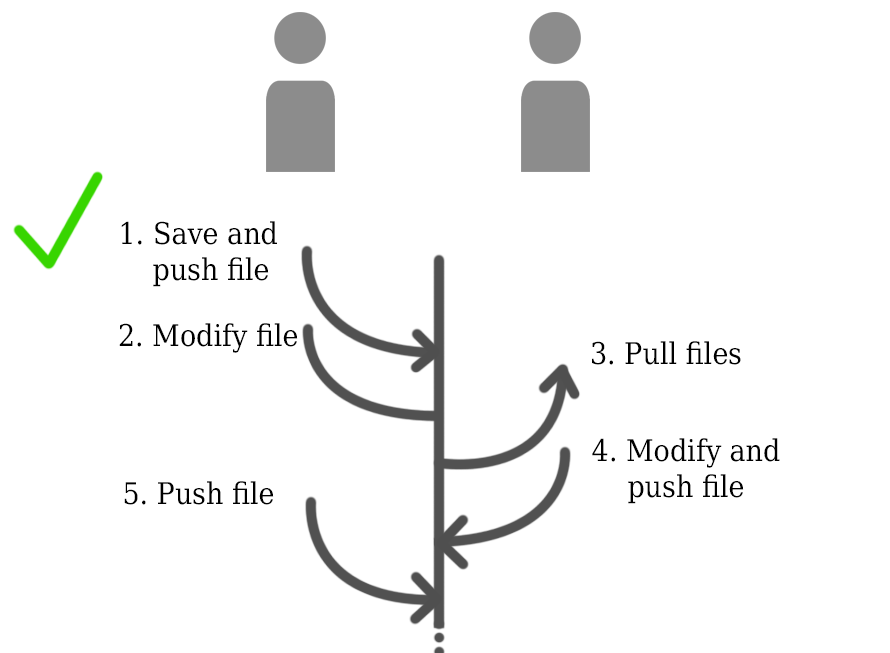
\includegraphics[width=0.9\textwidth]{VCS1}
	\end{figure}

}

\frame{ 
	\frametitle{Why do you want to use it?}
	
	\begin{figure}[hbtp]
		\centering
		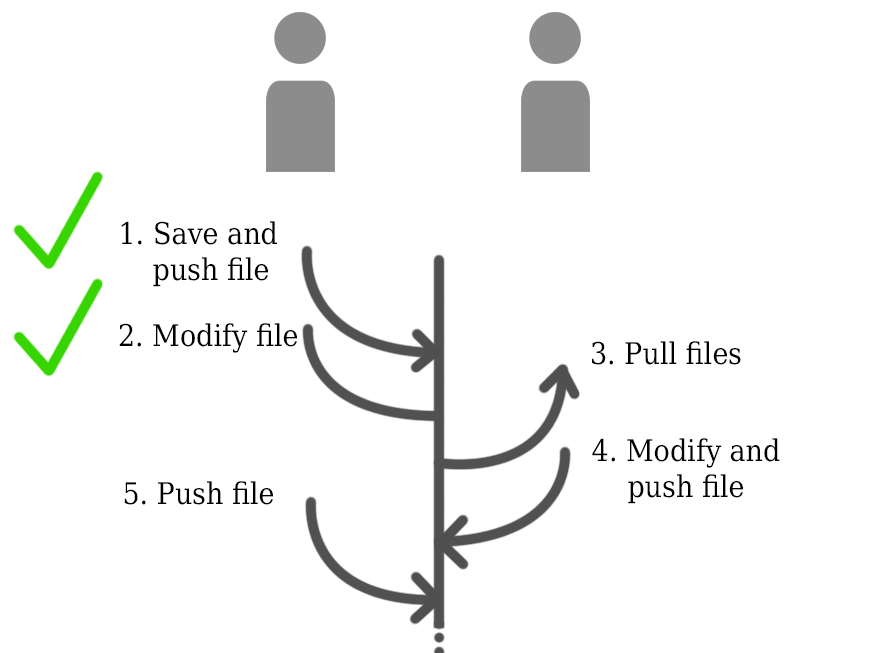
\includegraphics[width=0.9\textwidth]{VCS2}
	\end{figure}
	
}

\frame{ 
	\frametitle{Why do you want to use it?}
	
	\begin{figure}[hbtp]
		\centering
		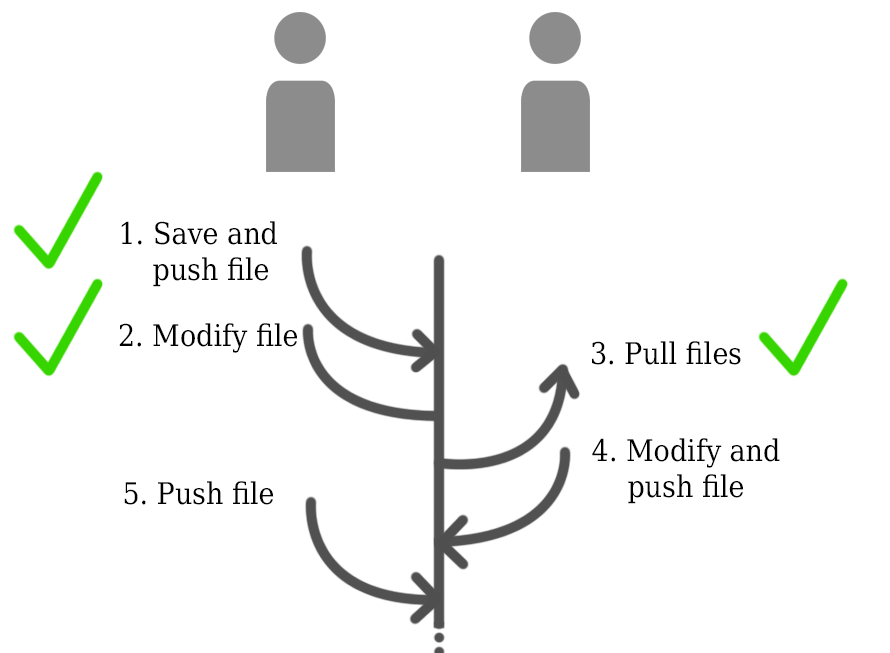
\includegraphics[width=0.9\textwidth]{VCS3}
	\end{figure}
	
}

\frame{ 
	\frametitle{Why do you want to use it?}
	
	\begin{figure}[hbtp]
		\centering
		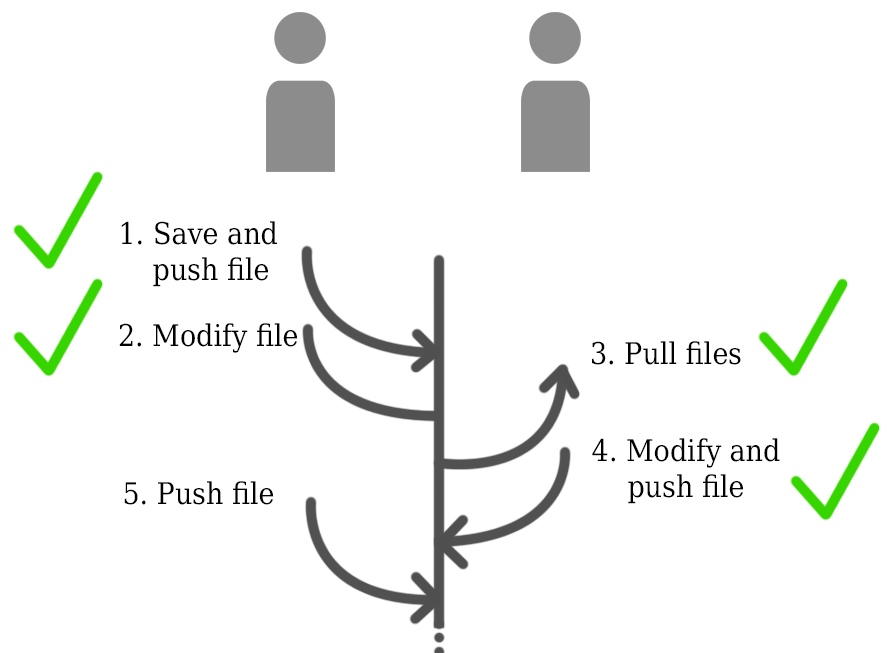
\includegraphics[width=0.9\textwidth]{VCS4}
	\end{figure}
	
}

\frame{ 
	\frametitle{Why do you want to use it?}
	
	\begin{figure}[hbtp]
		\centering
		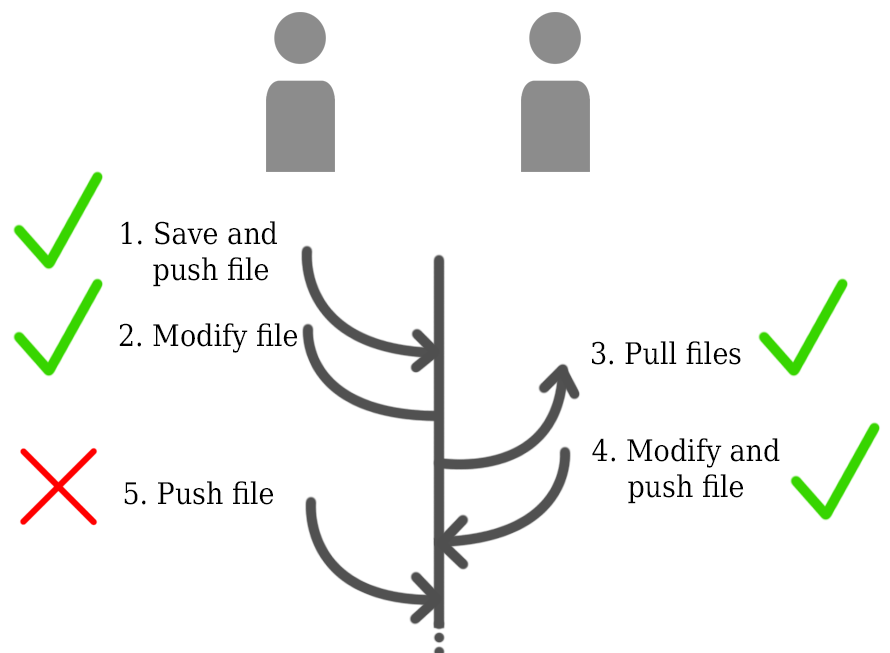
\includegraphics[width=0.9\textwidth]{VCS5}
	\end{figure}
	
}


\subsection{Merge}
\frame{ 
	\frametitle{Merge}
When conflicts occur they must be solved one way or another.
The most common way is to merge files.
\\
This is taking what was in the original file, the modified, compare them and bring the correct output.
	\begin{figure}[hbtp]
	\centering
	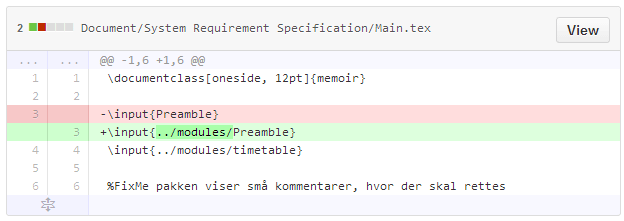
\includegraphics[width=0.95\textwidth]{Merge}
	\end{figure}
}


\section{How to get started}

\frame{
	\frametitle{How to get started}	
	
To get setup and running we will need the following:

\begin{itemize}
	\item Create a GitHub account.
	\item Download and install SmartGit.
	\item Setup SmartGit with GitHub.
	\item Create a small collaboral example.
\end{itemize}
}

\subsection{Create a GitHub account}
\frame{
\frametitle{Create a GitHub account}	

\begin{itemize}
	\item Go to \url{github.com}
	
	\item Create a user.
	\item[] Remember -- this name will be visible.
	
	\item Select a free plan. 
	
\end{itemize}
	
}

\subsection{Download and install SmartGit}

\frame{
\frametitle{Download and install SmartGit}

\begin{itemize}
	\item Download it from \url{http://www.syntevo.com/smartgit/download}
	\item Install SmartGit with the standard settings.
\end{itemize}	
}

\subsection{Setup SmartGit with GitHub.}

\frame{
	\frametitle{Setup SmartGit with GitHub.}
	
	\begin{itemize}
		\item Open the program.
		\item Select "Non-commercial use only".
		\item[] Confirm this.
		\item Select the second option for SSH with Git.
		\begin{itemize}
			\item Enter your GitHub account name.
			\item Click the "Generate API Token" key.
			\item Feel free whether to use a master password or not.
			\item[] It's security and will promt you after each reboot.
		\end{itemize}
		\item Finish the setup.

	\end{itemize}	
}

\frame{
	\frametitle{Setup SmartGit with GitHub.}
	
	\begin{itemize}
		\item Close the popup menu.
		\item Select from the menu bar \texttt{Tools} $\rightarrow$ 
		\texttt{Open Git-Shell}.
		\item Follow the link from step 1 with the Git-shell as terminal. 
		\\
		\textbf{DO NOT DOWNLOAD THE NATIVE APP}.
	\end{itemize}
	\url{https://help.github.com/articles/generating-ssh-keys}
		
}


\section{Live demo}
\frame{
\frametitle{Live demo}

Time for showing how this work.
We will go through the following:

\begin{itemize}
	\item Create a repository (project).
	\item Add collaborators to the repository.
	\item Add files to the repository, modify and push them (upload).
	\item Create a merge conflict and solve it properly.
	\item Create a list of files to ignore.
\end{itemize}
}



\end{document}

